\chapter{Fingering Arrangement}

\label{Chapter:Fingering-Arrangement}
\lhead{\emph{Fingering Arrangement}}

\section{Introduction}
A guitar consist of several parts. In this problem, we focus on the fretboard only.
Figure \ref{fig:guitar} shows names of the part that we interest about.

\begin{figure}[h]
    \centering
    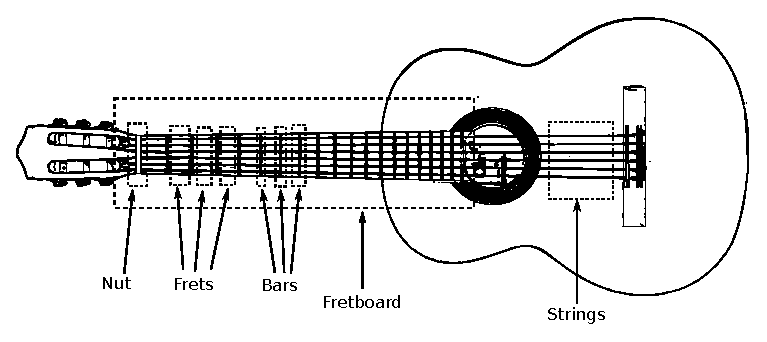
\includegraphics[width=\textwidth]{Figures/guitar.eps}
    \caption{Classical guitar}
    \label{fig:guitar}
\end{figure}

The fretboard can be viewed as a grid system split by 6 strings and 17(or more) bars. For consistence, we assume there is 17 bars on the fretboard. A grid can be described by the (fret, string) pair, where fret ranges from 0 to 17 and string ranges from 0 to 5. The frets count from left to right in Figure \ref{fig:guitar}, and strings count from top to bottom.

When playing the guitar, one use the left hand to press a grid, then use right hand to pluck the corresponding string, then a sound can be produced. Some sounds can be produced by plucking the string without pressing the grid since all strings are attached to the nut. This is so-called ``play by empty string''. We consider fret 0 is used in the empty string situation.

Four fingers in ones left hand are used for pressing the fretboard. Thumb is not used in this job, it is used to grip the neck of guitar. In our discussion, fingers of left hand are numbered into 0, 1, 2, 3, where 0 is for the index finger, and so on. A single finger can press only one grid at a time, except the index finger. We can use the index finger to press more than one grid at a time. This technique is called ``baring''. It cannot be used in every combination of grids. Instead, it can only be used to press the grids on the same fret and a consecutive range of strings. Figure \ref{fig:fretboard-baring} shows an example of the baring technique.

\begin{figure}[h]
    \centering
    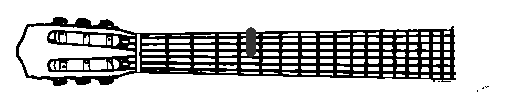
\includegraphics[width=0.6\textwidth]{Figures/fretboard-baring.eps}
    \caption{Baring by the index finger.}
    \label{fig:fretboard-baring}
    \startdescription
    In this example, fret 5 of strings (0, 1, 2) is pressed by the index finger.
\end{figure}

Normally, without special techniques, each grid on the fretboard can only produce a specific
pitch of sound. For example, The grid (5, 0) can produce sound A4(440Hz) and grid (1, 0) can produce C4. Table \ref{table:standard-tuning} shows the pitch that can be produced by each grid on the fretboard. From this table we see that the pitches on the same string are ascending uniformly. Once the pitch of grid (0, $i$) is known to be $p_i$, the pitch of grid ($f$, $i$) can be calculated by $p_i + f$.

\begin{table}
    \centering
    \tiny \tabcolsep=0.05cm
\begin{tabular*}{\textwidth}{r|c|c|c|c|c|c|c|c|c|c|c|c|c|c}
& 0& 1& 2& 3& 4& 5& 6& 7& 8& 9& 10& 11& 12& 13\\ \hline
0
& E4(64)& F4(65)& F\#4(66)& G4(67)& G\#4(68)& A4(69)& A\#4(70)& B4(71)& C5(72)& C\#5(73)& D5(74)& D\#5(75)& E5(76)& F5(77)\\ \hline
1
& B3(59)& C4(60)& C\#4(61)& D4(62)& D\#4(63)& E4(64)& F4(65)& F\#4(66)& G4(67)& G\#4(68)& A4(69)& A\#4(70)& B4(71)& C5(72)\\ \hline
2
& G3(55)& G\#3(56)& A3(57)& A\#3(58)& B3(59)& C4(60)& C\#4(61)& D4(62)& D\#4(63)& E4(64)& F4(65)& F\#4(66)& G4(67)& G\#4(68)\\ \hline
3
& D3(50)& D\#3(51)& E3(52)& F3(53)& F\#3(54)& G3(55)& G\#3(56)& A3(57)& A\#3(58)& B3(59)& C4(60)& C\#4(61)& D4(62)& D\#4(63)\\ \hline
4
& A2(45)& A\#2(46)& B2(47)& C3(48)& C\#3(49)& D3(50)& D\#3(51)& E3(52)& F3(53)& F\#3(54)& G3(55)& G\#3(56)& A3(57)& A\#3(58)\\ \hline
5
& E2(40)& F2(41)& F\#2(42)& G2(43)& G\#2(44)& A2(45)& A\#2(46)& B2(47)& C3(48)& C\#3(49)& D3(50)& D\#3(51)& E3(52)& F3(53)\\ \hline
\end{tabular*}
    \caption{Fretboard pitch table on standard tuning}
    \label{table:standard-tuning}
    \startdescription
    Number in the parentheses are the midi pitch level.
\end{table}

The problem of fingering arrangement is to assign a grid and a finger for each desired notes that we want to produce. 

In Table \ref{table:standard-tuning}, we can see that different grids may produce same pitch. For example, both grids (5, 5) and (0, 4) can produce A2, and both grids (1, 1), (5, 2), (10, 3), (15, 4) can produce C4. Actually, almost every pitch can be produced by more than one grid. Also, different grids can be pressed by different fingers. All these make it impractical to  enumerate all possible combinations to find the optimal solution. By optimal we mean the one that is most easy to play. This will be defined formally in the next section.

\section{Model}
In this problem, we describe a note by (pitch, start time, end time). The solution to the problem should resolve each note by assigning a (finger, fret, string). Since a note can also be played by empty string, the finger value in (finger, fret, string) tuple may equal to -1, which means no finger. 
\[
\mathrm{fingerings} \gets \mathrm{Arrange}(\mathrm{noteSequence})
\]

\subsection{Key Times}
A key time is a time that one or more notes start. Key times are important because all the finger movements start at key time. The first step to solve this problem is to extract all start times from the note sequence as the key time collection. The key time collection is a sequence of different key times.

\subsection{Frame}
A frame at time $t$ is defined as the collection of notes whose time interval contains $t$. More formally, suppose the note is represented by $(p, t_1, t_2)$, and the note sequence is denoted by $N$, then the frame is \[
\mathrm{frame(t)} = \left\{ (p, t_1, t_2) | (p, t_1, t_2) \in N, t_1 \le t < t_2 \right\}
\]
In our method, only frames at key times are interested. All frames are generated by a scanning algorithm, which is described in Algorithm \ref{algo:gen-frames}. First we convert the notes into note events, as we do in chapter \ref{Chapter:Playing-Sound}. Then during the scanning process, we use a list to keep track of the active note events. At time $t$, from the active events we know the notes in the current frame.

\begin{algorithm}[h]
    \caption{Generate Frames} \label{algo:gen-frames}.
    \begin{algorithmic}
        \Function{Generate Frames}{$T$, $E$} \Comment{$T$ is the key time sequence. $E$ is the note event sequence.}
            \Require $E$ is sorted by start time.
            \State F $\gets$ empty set \Comment{The frame sequence.}
            \State $E_a$ $\gets$ empty list \Comment{Active events.}
            \State $p \gets 0$
            \For {$t \in T$}
                \State $E_a \gets \left\{e | e \in E_a, e.\mathrm{end} > t \right\}$
                \While {$p < \mathrm{length}(E)$ and $E(i).\mathrm{start} == t$}
                    \State Append $E(i)$ to $E_a$
                    \State $p \gets p + 1$
                \EndWhile
            \EndFor
            \State make a frame using $E_a$ and then append it to $F$
            \State \Return $F$
        \EndFunction

    \end{algorithmic}
\end{algorithm}

\subsection{Play State}
A play-state at time $t$ describes the state of the left hand and the ringing strings. With these information, we will be able to calculate the cost at time $t$ or cost between two successive key time.

A play-state can be represented by \[ (b, F(i), S(i), R(j)) \] Where $b$ tells this state is barring or not; $F$ and $S$ are functions and their domain is the finger collection ${0, 1, 2, 3}$. In this state, finger $i$ is pressing the grid $(F(i), S(i))$. $R$ is also a function and its domain is the string collection ${0, 1, 2, 3, 4, 5}$. $R(j) = \mathrm{True}$ means that in this state, string $j$ is used.

In our method only play-states at key times are interested. 
A valid play-state for time $t$ is  a play-state that can produce all notes in $\mathrm{frame}(t)$. At each key time, we may have multiple valid play-states.  The solution of the fingering arrangement problem can be described by a sequence of play-states. In such a solution, a play-state is chosen for each key time. 

Suppose in a solution, play-state $S_i$ is assigned to the $i$-th key time $t_i$. Since a play-state tells us all information about how to put the left hand, knowing $S_i$ and $S_{i+1}$ is sufficient to let the player move the left hand. The cost at all play-state $S_i$, and between all $S_i$, $S_{i+1}$ pairs, are summed up to get the total cost for this solution, using equation \ref{eqn:solution-cost}.
\begin{eqnarray}
    & \mathrm{SolutionCost}(
        \left\{t_0, t_1, \cdots, t_n\right\}, \left\{S_0, S_1, \cdots, S_n\right\}
    )  \nonumber\\
    =& \sum_{i = 0}^n C_{\mathrm{static}}(S_i)
    + \sum_{i = 0}^{n - 1} C_{\mathrm{transition}}(t_i, t_{i+1}, S_i, S_{i+1})
    \label{eqn:solution-cost}
\end{eqnarray}

The cost functions $C_{\mathrm{static}}(S_i)$ and $C_{\mathrm{transition}}(t_i, t_{i+1}, S_i, S_{i+1})$ will be discussed in section \ref{section:cost-function}.

\subsection{State Transition Equation}
We use a dynamic programming method to find the play-states solution. 

Let $C(t_i, S)$ be the minimum cost to stay at play-state $S$ at key time $t_i$. Then we can calculate $C(t_i, S)$ using dynamic programming.
All valid play-state for each frame is generated before we calculate $C(t_i, S)$.  We denote the valid play-state for frame at time $t_i$ as $V_i$.

\begin{eqnarray}
    C(t_i, S) = C_{\mathrm{static}}(S) +
        \min_{S' \in V_{i-1}} \left[
            C(t_{i-1}, S') + 
            C_{\mathrm{transition}}(t_{i-1}, t_i, S', S) 
        \right]
    \label{eqn:transition}
\end{eqnarray}
Our goal is to find the play-state $S$ such that $C(t_n, S)$ has the minimum value. Once we got such an $S$,  we can trace back the play-state sequence by the decision on every step to get the corresponding play-state sequence. 


\section{Generating Valid play-state}
A play-state is considered valid if and only if it's playable. Human hand has physical constraint, so some of the grid combinations are impossible to play. Suppose we now have a play-state $S=(b, F(i), S(i), R(j))$, the constraints are listed below.
\begin{enumerate}
    \item For any $i, j, i \le j$, we have $F(i) \le F(j)$.
    \item For any $i, j, i \neq j$, we have $S(i) \neq S(j)$.
    \item For any $i, j, i \le j \land F(i) = F(j)$, we have $S(i) > S(j)$.
    \item When $b = True$, then for any $i > 0$, we have $F(i) > F(0)$.
    \item Fingers should not be too far away from index finger.
    \item When $b = True$, fingers should not be too close from index finger.
\end{enumerate}

Here we set the constraint distance value to maximum or minimum distance that our hand can stretch. The values we used in our implementation are listed in Table \ref{table:finger-constraints}.

\begin{table}[h]
    \centering
    \begin{tabular}{r|r|r|r}
        Fingers & 1 & 2 & 3 \\
        \hline
        max & 0.06 & 0.10 & 0.13 \\
        min & 0.008 & 0.025 & 0.025 \\
    \end{tabular}
    \caption{Finger constraint distance values(in meters).}
    \label{table:finger-constraints}
\end{table}

To calculate the distance between any two grids, we need to know every bar positions. A guitar produces sound by the vibration of strings. When a string is pressed onto the fretboard, its length that contribute to the sound generation is effectively shortened. The frequency of the sound that a string produced is proportional to the multiplicative inverse of the effective length of the string. From the design of guitar, we know that the position of the 12th bar is in the exactly middle of a string. If the length of a string is $L$, then the distance $d_i$ of the $i$-th bar can be calculated by solving equations \ref{eqn:fretboard-proportional}.
\begin{eqnarray}
    \left\{
    \begin{aligned}
        l_i &=  L - d_i \\
        l_{12} &=  L - \frac{L}{2} \\
        l_i p_i &=  l_{12} p_{12} \\
        p_i &=  p_{12} (\sqrt{2})^{ \frac{i}{12}}
    \end{aligned}
    \label{eqn:fretboard-proportional}
    \right.
\end{eqnarray}

Solving these equations we got \[ d_i = (1 - 2^{-i/12})L \]
With this formula we can calculate the distance of any pair of grids.

To generate all valid states for a frame efficiently, we use the strategy that removes the invalid states as early as possible. First, the fret for index finger is chosen. With the index finger chosen, the remaining search space become much smaller. Then we choose to use the index finger or not. Even if the index finger is not used, the fret position of it can describe the hand position. If the index finger is used, a string will be assigned to it. After these steps, the search space is small enough so we can use a brute force recursive searching method to resolve the remaining notes.At each level of recursion, we resolve a note at current frame, and then test the validness according to the constraints. If all the notes are resolve at some level, we start to assign fingers to the used grids. Finally, a new valid play-state is generated.

\section{Cost Function} \label{section:cost-function}
We have two types of cost functions. The first type is the static cost function. The other type is transition function. Static cost is only relevant to frame and play-state at a single key time, while transition cost is relevant to two key times. 

\subsection{Static Cost}
Static cost function consists of two parts: the ``missing penalty'' and the ``high fret penalty''. Missing notes in a play-state is heavily penalized. A note is considered missing in a play-state when it's not resolved by the state. In Figure \ref{fig:guitar}, we can see that frets higher than the 12th bar is on the front surface of the guitar. This make it more difficult to use the frets there, because there's no place for the thumb to grip the neck(it's out of the neck!). Therefore, we have penalty on high frets. In our implementation, fret higher than 9 are considered high. Summarizing these two types of cost, and suppose play-state to be $(b, F, S, R)$  we get:
    \[
    C_{\mathrm{static}}(S) = n_{\mathrm{miss}} K_{\mathrm{miss}} 
        + \sum_{F(i) > F_{\mathrm{high}}} (F(i) - F_{\mathrm{high}}) K_{\mathrm{high}}
    \]
Where $K_{\mathrm{miss}}$ and $K_{\mathrm{high}}$ are constants we got by experiment. 

\subsection{Transition Cost}
Transition cost describes the cost when the hand translates from one state to another state. It can be calculated by summing the movement cost of the arm and the movement cost of each finger. Suppose we are to calculate $C_{\mathrm{transition}}(t_1, t_2, S_1, S_2)$.
The predicate function $P(S, i)$ tells if finger $i$ is pressed in play-state $S$. Then, for finger $i$ from fingers other than index, we observe these 4 situations: 
\begin{description}
    \item[$\lnot P(S_1, i) \land \lnot P(S_2, i)$] \hfill \\
        A free transition, finger $i$ is not used in both play-state. No cost to add.

    \item[$\lnot P(S_1, i) \land P(S_2, i)$] \hfill \\
        Finger $i$ need to pressed on the grid $(F_2(i), S_2(i))$ before time $t_2$. From $S_1$ we can know that when should string $S_2(i)$ stop, then we can calculate the time $\Delta t$ the finger can use to press.
        Add $K_{\mathrm{press}} / \Delta t$ to total cost.

    \item[$P(S_1, i) \land P(S_2, i)$] \hfill \\
        The finger is pressing some grid in both states. Note that the grids it press may be the same or different. If they are the same, add $K_{\mathrm{keep}}(t_2 - t_1)$ to total cost. If they are different, the finger is moved from grid $(F_1(i), S_1(i))$ to $(F_2(i), S_2(i))$,
        so we add \[
        K_{\mathrm{movefret}} \left[ (F_1(i) - F_1(0)) - (F_2(i) - F_2(0)) \right]^2
        + K_{\mathrm{movestring}} \left( S_1(i) - S_2(i)\right)^2
        \]

    \item[$P(S_1, i) \land \lnot P(S_2, i)$] \hfill \\
        Finger $i$ should be released before time $t_2$. The time interval $\Delta t$ that the finger can use to release is calculated similar to the one we use to calculate pressing time. Add $K_{\mathrm{release}} / \Delta t$ to total cost.
\end{description}

For the index finger, which has three states, the cost calculation is similar, but a bit more complexed. It has 9 situations but some are overlapped with the normal fingers'. We are not going to list them here.

One other cost is the missing penalty. If a note is in both frames at $t_1$ and $t_2$, and is resolved by different grid or finger, then this note is considered missing. This is because we cannot keep the string vibrating when switching to another finger. This kind of missing is also penalized by
$n_\mathrm{miss} K_\mathrm{miss}$.


\section{Decision Process}

From equation \ref{eqn:transition}, we can see that once we know all $C(t_{i-1}, S')$ for any 
$S'$, we are able to calculate $C(t_i, S)$. $C(t_0, S)$ is calculated by taking only the static cost.
Using math induction, we can calculate $C(t_n, S)$ for any $S$. Finally we got Algorithm \ref{algo:dp}

\begin{algorithm}
    \caption{Calculate Cost} \label{algo:dp}
    \begin{algorithmic}
    \Procedure {Calculate Cost}{$T$, $F$}
        \State \Comment{$T$: key times, $F$: key frames}
        \State Generate valid states $V_i$ for each frame $F_i$.
        \State D $\gets$ empty table \Comment Choice table
        \State C $\gets$ empty table \Comment Cost table
        \For {$S \in V_0$} 
            \State $C(t_0, S) \gets C_{\mathrm{static}(S)}$
        \EndFor
        \For {$i \in [1, n]$}
            \For {$S \in V_i$}
                \State $C(t_i, S) \gets \min_{S' \in V_{i-1}} \left[
                        C(t_{i-1}, S') + C_{\mathrm{transition}}(t_{i-1}, t_i, S', S)
                    \right] $
                \State $D(t_i, S) \gets \argmin_{j, S_j \in V_{i-1}} \left[
                        C(t_{i-1}, S_j) + C_{\mathrm{transition}}(t_{i-1}, t_i, S_j, S)
                    \right] $
            \EndFor
        \EndFor
    \EndProcedure
    \end{algorithmic}
\end{algorithm}

Aside from calculating the minimum value, the corresponding choices are also saved. Using these choices, we can recover the corresponding play-state sequence, which is our goal to the fingering arrangement problem.

In this algorithm, both time and space complexity are $O(nm^2)$, where $m$ is the average number of
valid states for each frame. By experiment, we found that $n$ is usually 500 to 1000, and $m$ varies from 1 to 100.

One important optimization for the decision algorithm, is to rearrange the order of all available $S'$ so that unnecessary are decreased. For each $C(t_i, S)$, we make a copy of $V_{i-1}$, then sort it by the delta index fret. When current minimum value is less than the minimum possible value of each remaining candidate play-state $S'$, there's no need to compare for these candidates. The optimized algorithm is shown in Algorithm \ref{algo:dp-optimized}

\begin{algorithm}
    \caption{Calculate Cost} \label{algo:dp-optimized}
    \begin{algorithmic}

    \Procedure {Calculate Cost}{$T$, $F$}
        \State \Comment{$T$: key times, $F$: key frames}
        \State Generate valid states $V_i$ for each frame $F_i$.
        \State D $\gets$ empty table \Comment Choice table
        \State C $\gets$ empty table \Comment Cost table
        \For {$S \in V_0$} 
            \State $C(t_0, S) \gets C_{\mathrm{static}(S)}$
        \EndFor
        \For {$i \in [1, n]$}
            \For {$S \in V_i$}
                \State $C(t_i, S) \gets +\infty$
                \State order $\gets$ $\left( 0, 1, \ldots, |V_{i-1}| \right)$
                \State order.sort(key=lambda $j$: $C(t_{i-1}, V_{i-1, j})
                        + \mathrm{delta fret cost}(V_{i-1, j}, S)$)
                \For {$j \in \mathrm{order}$}
                    \State $S' \gets V_{i-1, j}$
                    \If{$C(t_{i-1}, S') + \mathrm{delta fret cost(S', S)} \ge C(t_i, S)$}
                        \State break
                    \EndIf
                    \State $x \gets C(t_{i-1}, S') + 
                            C_{\mathrm{transition}}(t_{i-1}, t_i, S', S)$
                    \If{$x < C(t_i, S)$}
                        \State $C(t_i, S) \gets x$
                        \State $D(t_i, S) \gets j$
                    \EndIf
                \EndFor
            \EndFor
        \EndFor
    \EndProcedure
    \end{algorithmic}
\end{algorithm}


\section{Results}
% Scores:
%   Giuliani_-_Op.50_No.1.mxl
%   Pavane_No._6_for_Guitar_Luis_Milan.mxl
%   Lagrima.mxl
%   Lute_Suite_No._1_in_E_Major_BWV_1006a_J.S._Bach.mxl

We choose 4 classical guitar pieces and have our method tested upon them. For each piece, we cut 
some measures out and run our program to get the fingering. Then we generate the tablature and put them together with the origin scores. In our method, each note is assigned a finger for it. However, due to the limit of tablature, the finger is not label in the result score. 

These results are in Figure \ref{fig:result-lag}, \ref{fig:result-giu}, \ref{fig:result-lut} and \ref{fig:result-pav}.  These test cases are chosen to test the performance of our algorithm on different musical style.

Lágrima in \ref{fig:result-lag} is slower piece. Since the cost functions are time-relevant, we should its performance on pieces of different speed.

Giuliani Op.50 No.1 in \ref{fig:result-giu}  has two part of sound. The treble is fast and its every notes can be group to a chord. The right way to play this style is to have the left hand keep pressing the chord for each group of notes. In our result, this is arranged properly.

Lute Suite No.1 in E Major in \ref{fig:result-lut} is even faster than the Giuliani Op.50. However, its notes on treble part is not consists of chords. To play it properly, the left hand need to change quite a lot. Since it is so fast that the successive note with different pitch should better be played on different strings to decrease the burden of the left hand. If several successive notes are played on the same string, the left hand finger will have less time to press. The $\Delta t_\mathrm{press}$ in our cost model can reflect this situation.

Pavane No.6 for Guitar by Luis Milan in \ref{fig:result-pav} is a slow piece. However, it's actually more difficult to play since the notes on it are dense due to the extensive use of chords. For example, the first measure of it has 3 beats and each beat has a chord that consists of four notes. We can see that the fingering arrangement of our result is proper and playable.

\begin{figure}[h]
    \centering
    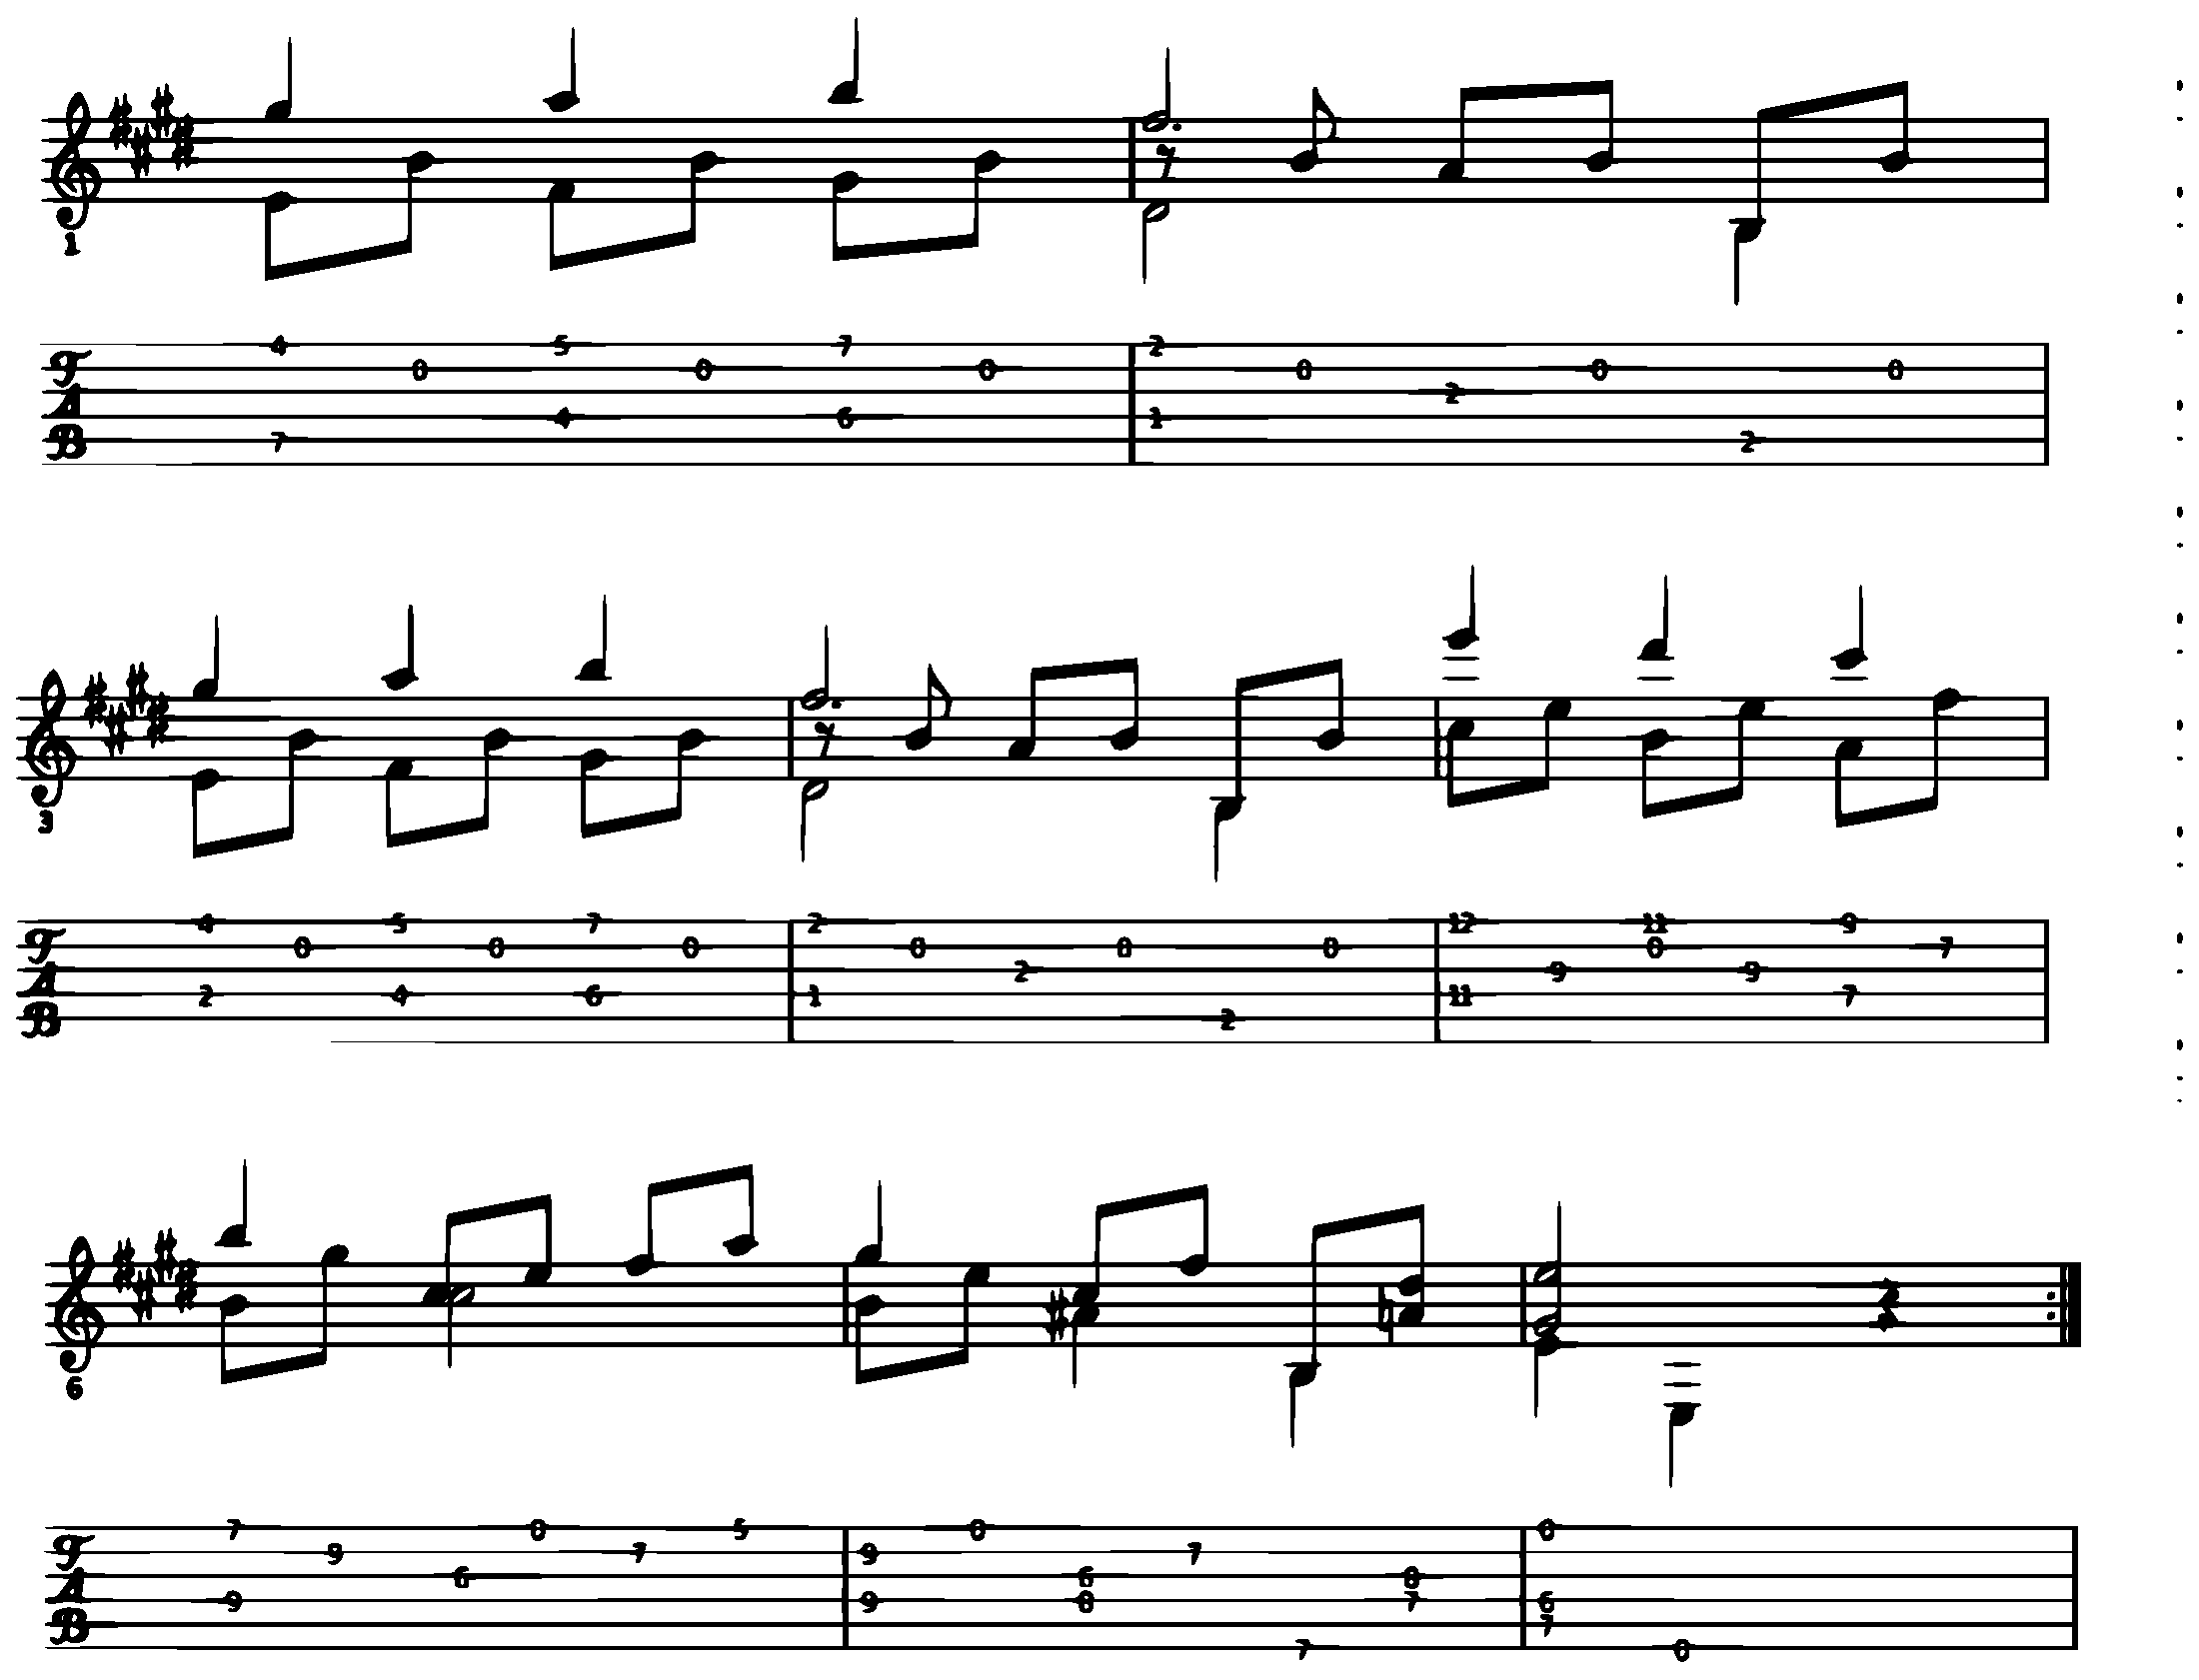
\includegraphics[width=1.0\textwidth]{Figures/Lag.eps}
    \caption{Lágrima by Francisco TÁRREGA}
    \label{fig:result-lag}
\end{figure}

\begin{figure}[h]
    \centering
    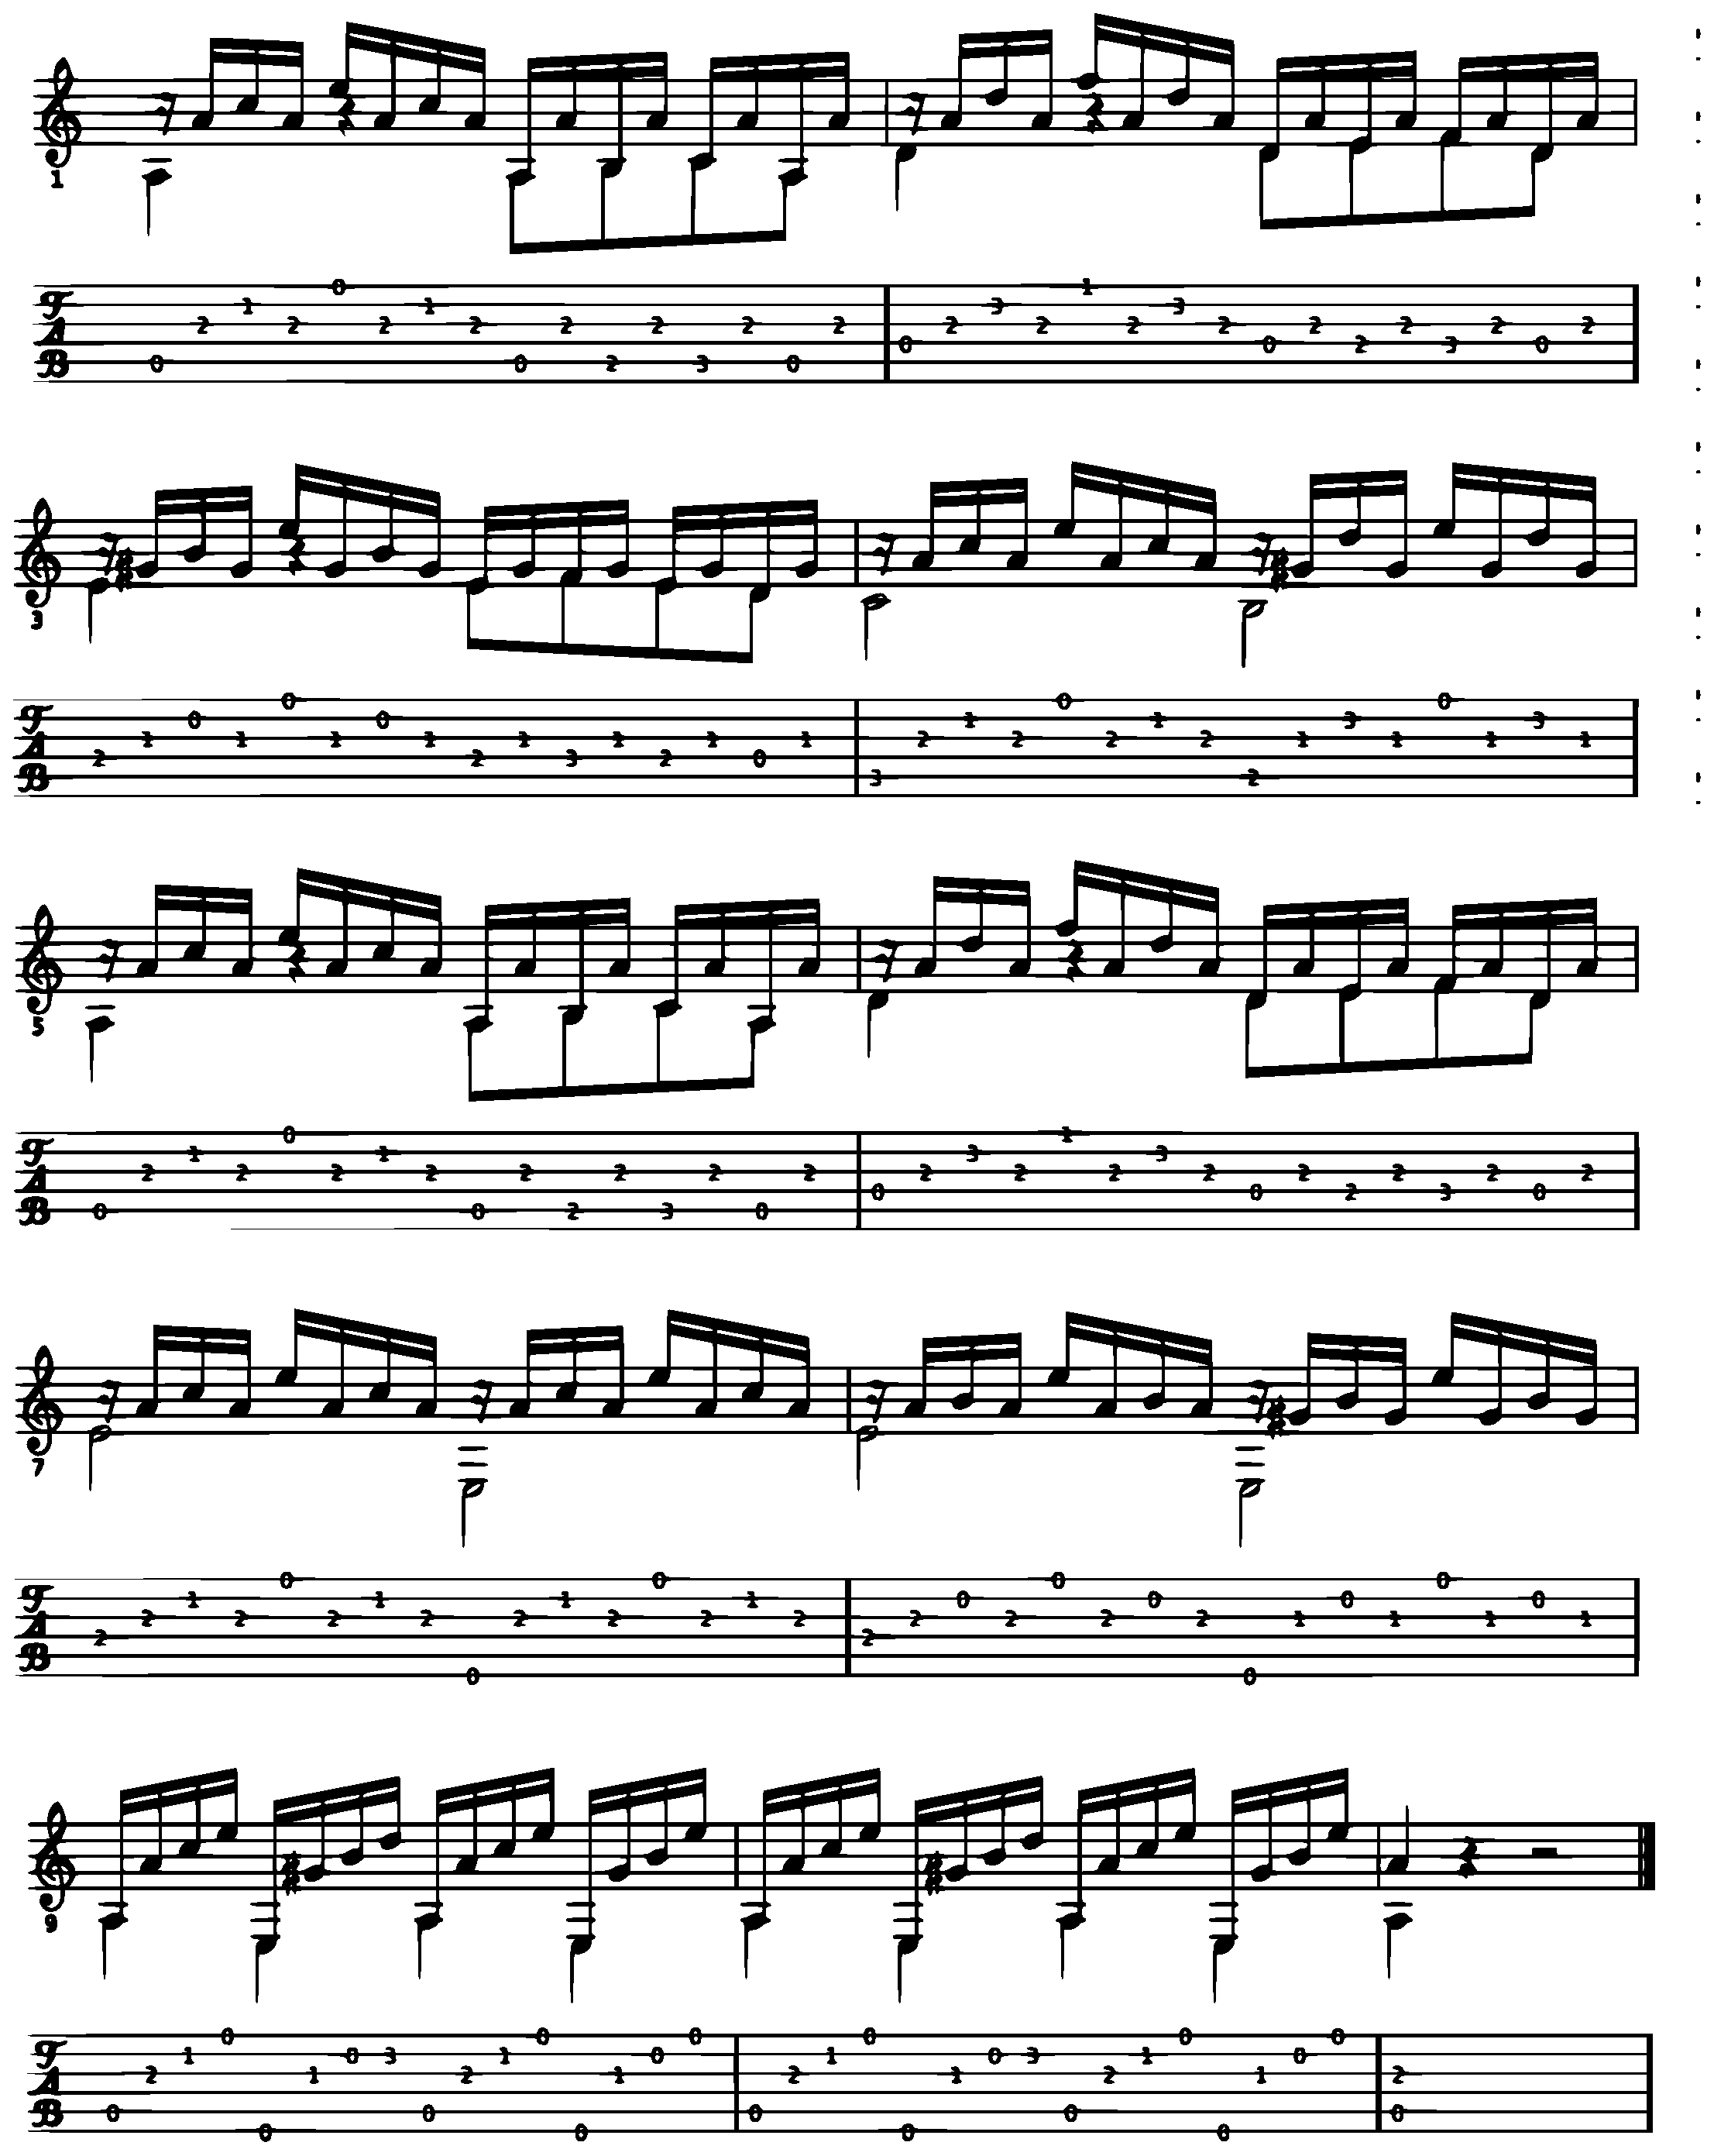
\includegraphics[width=1.0\textwidth]{Figures/Giu.eps}
    \caption{Giuliani Op.50 No.1}
    \label{fig:result-giu}
\end{figure}

\begin{figure}[h]
    \centering
    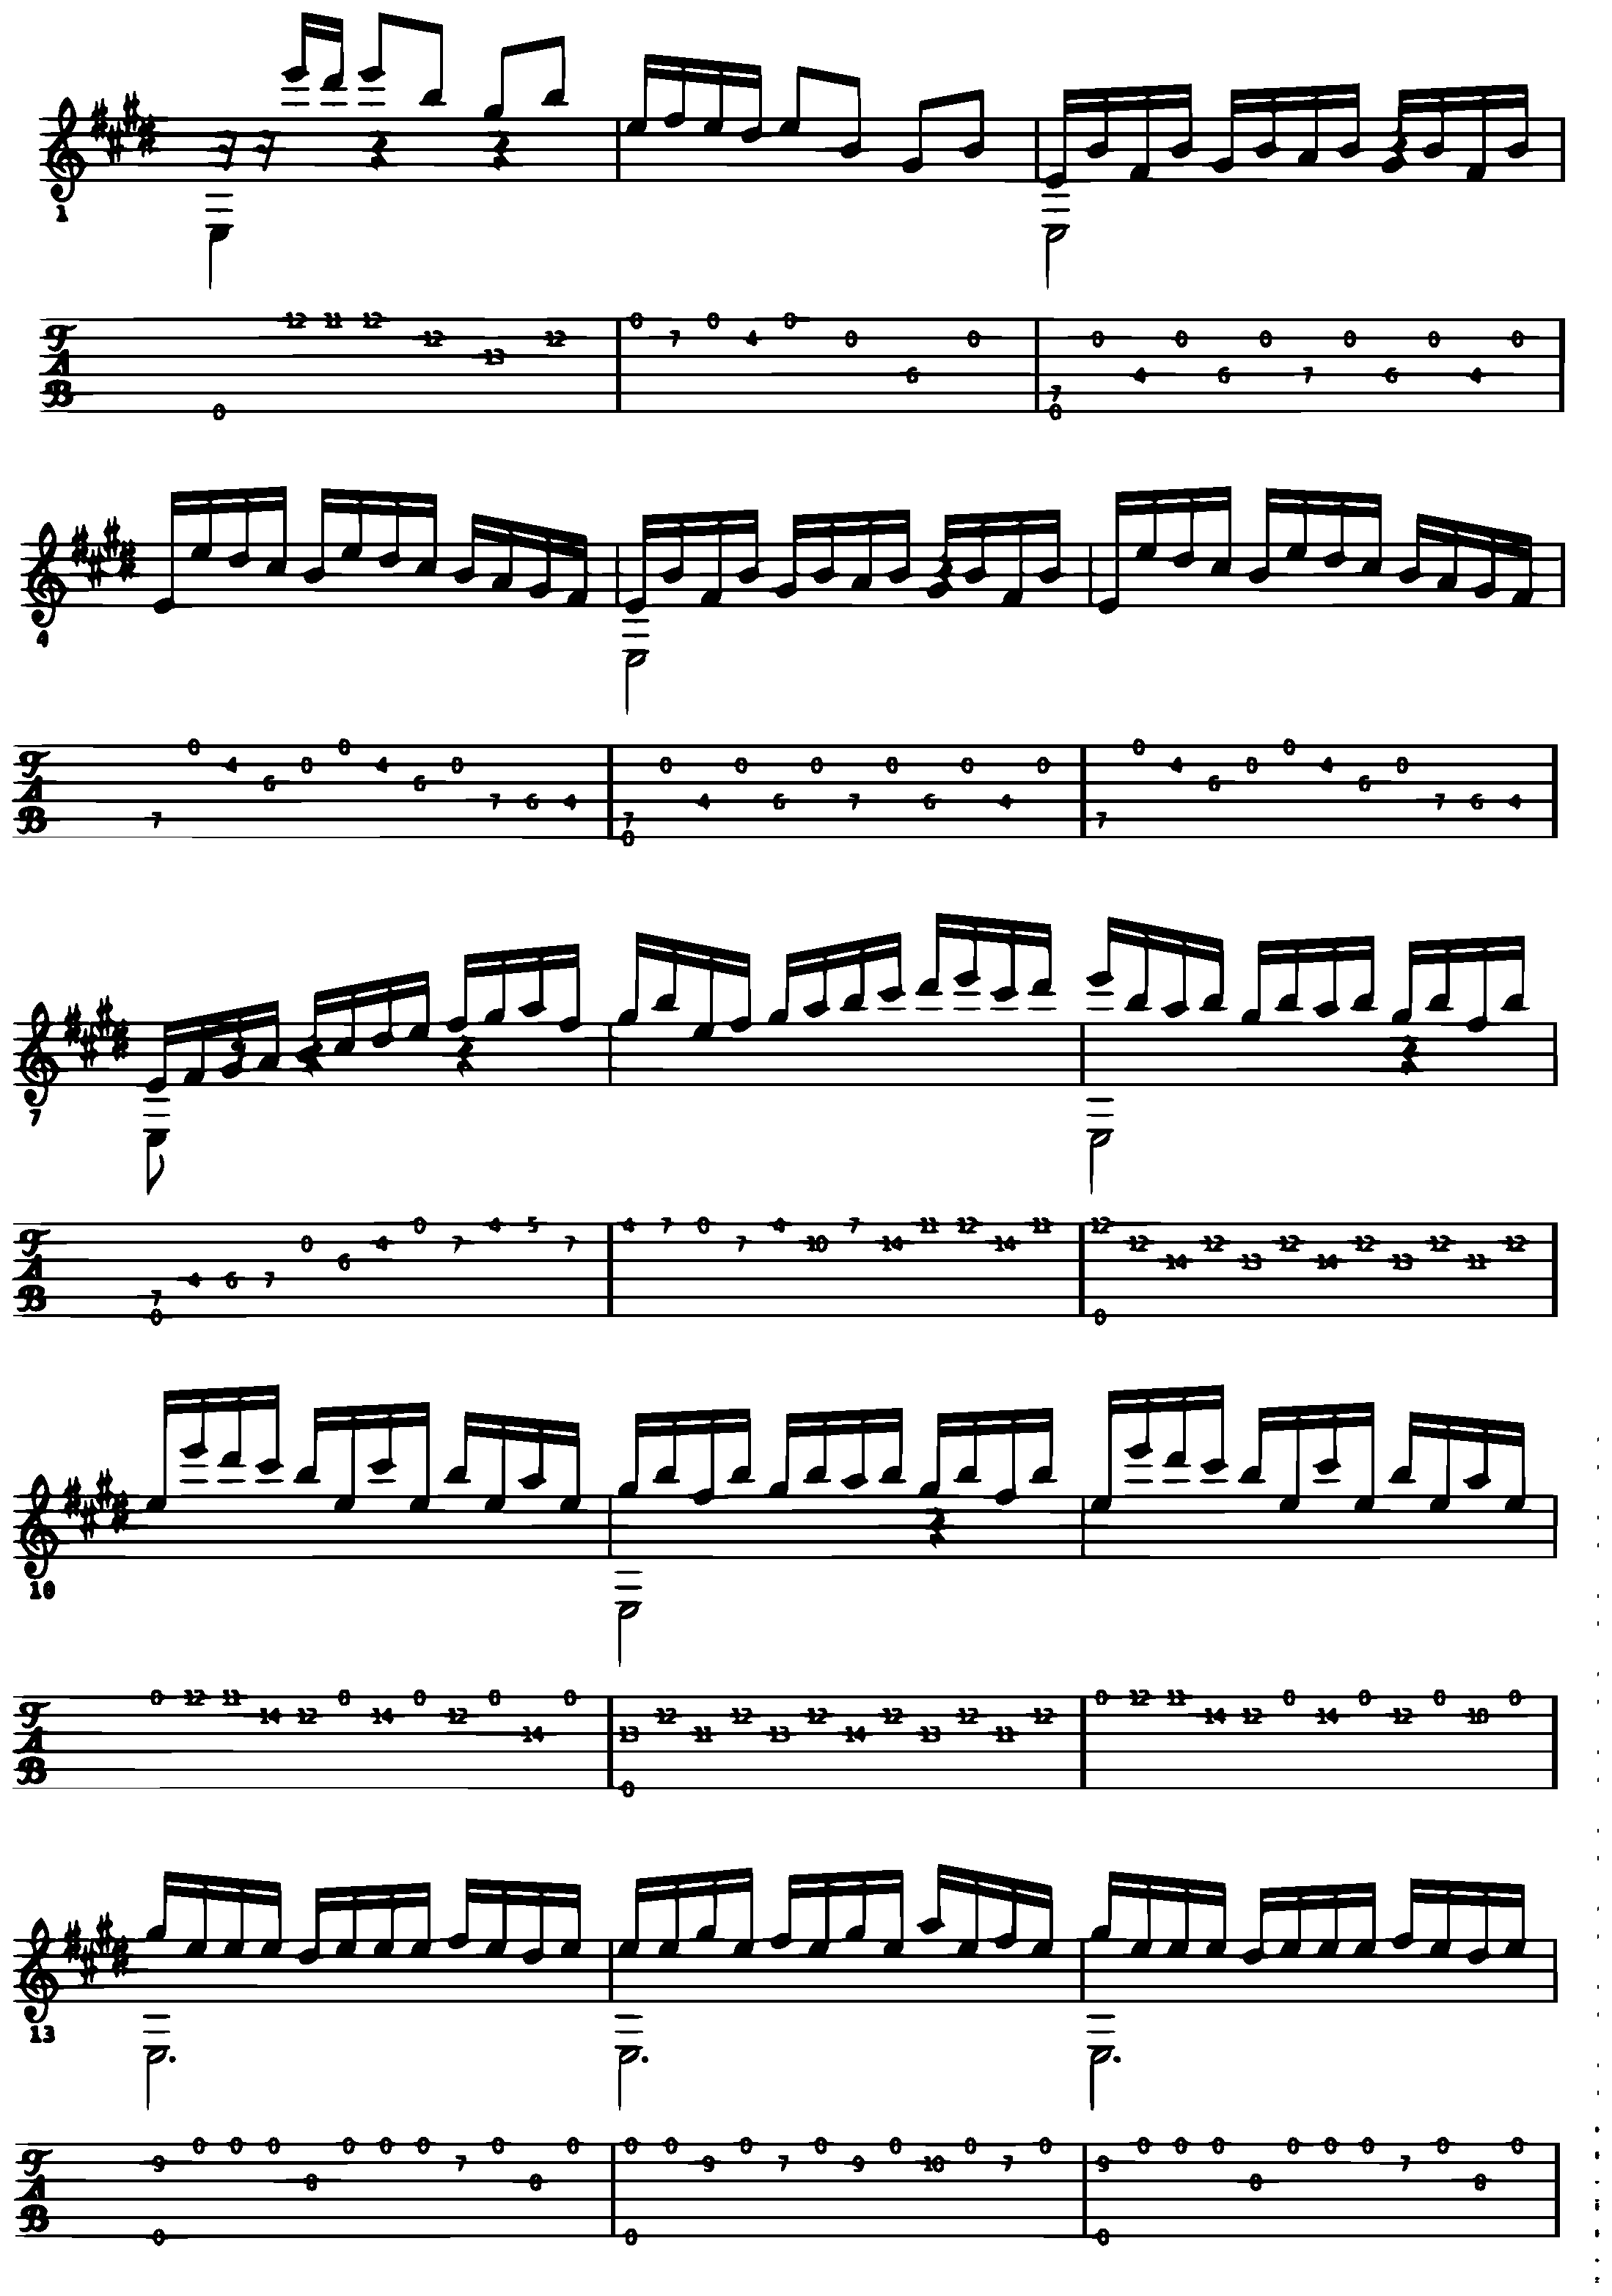
\includegraphics[width=1.0\textwidth]{Figures/Lut.eps}
    \caption{Lute Suite No.1 in E Major BWV 1006a by J.S. Bach}
    \label{fig:result-lut}
\end{figure}

\begin{figure}[h]
    \centering
    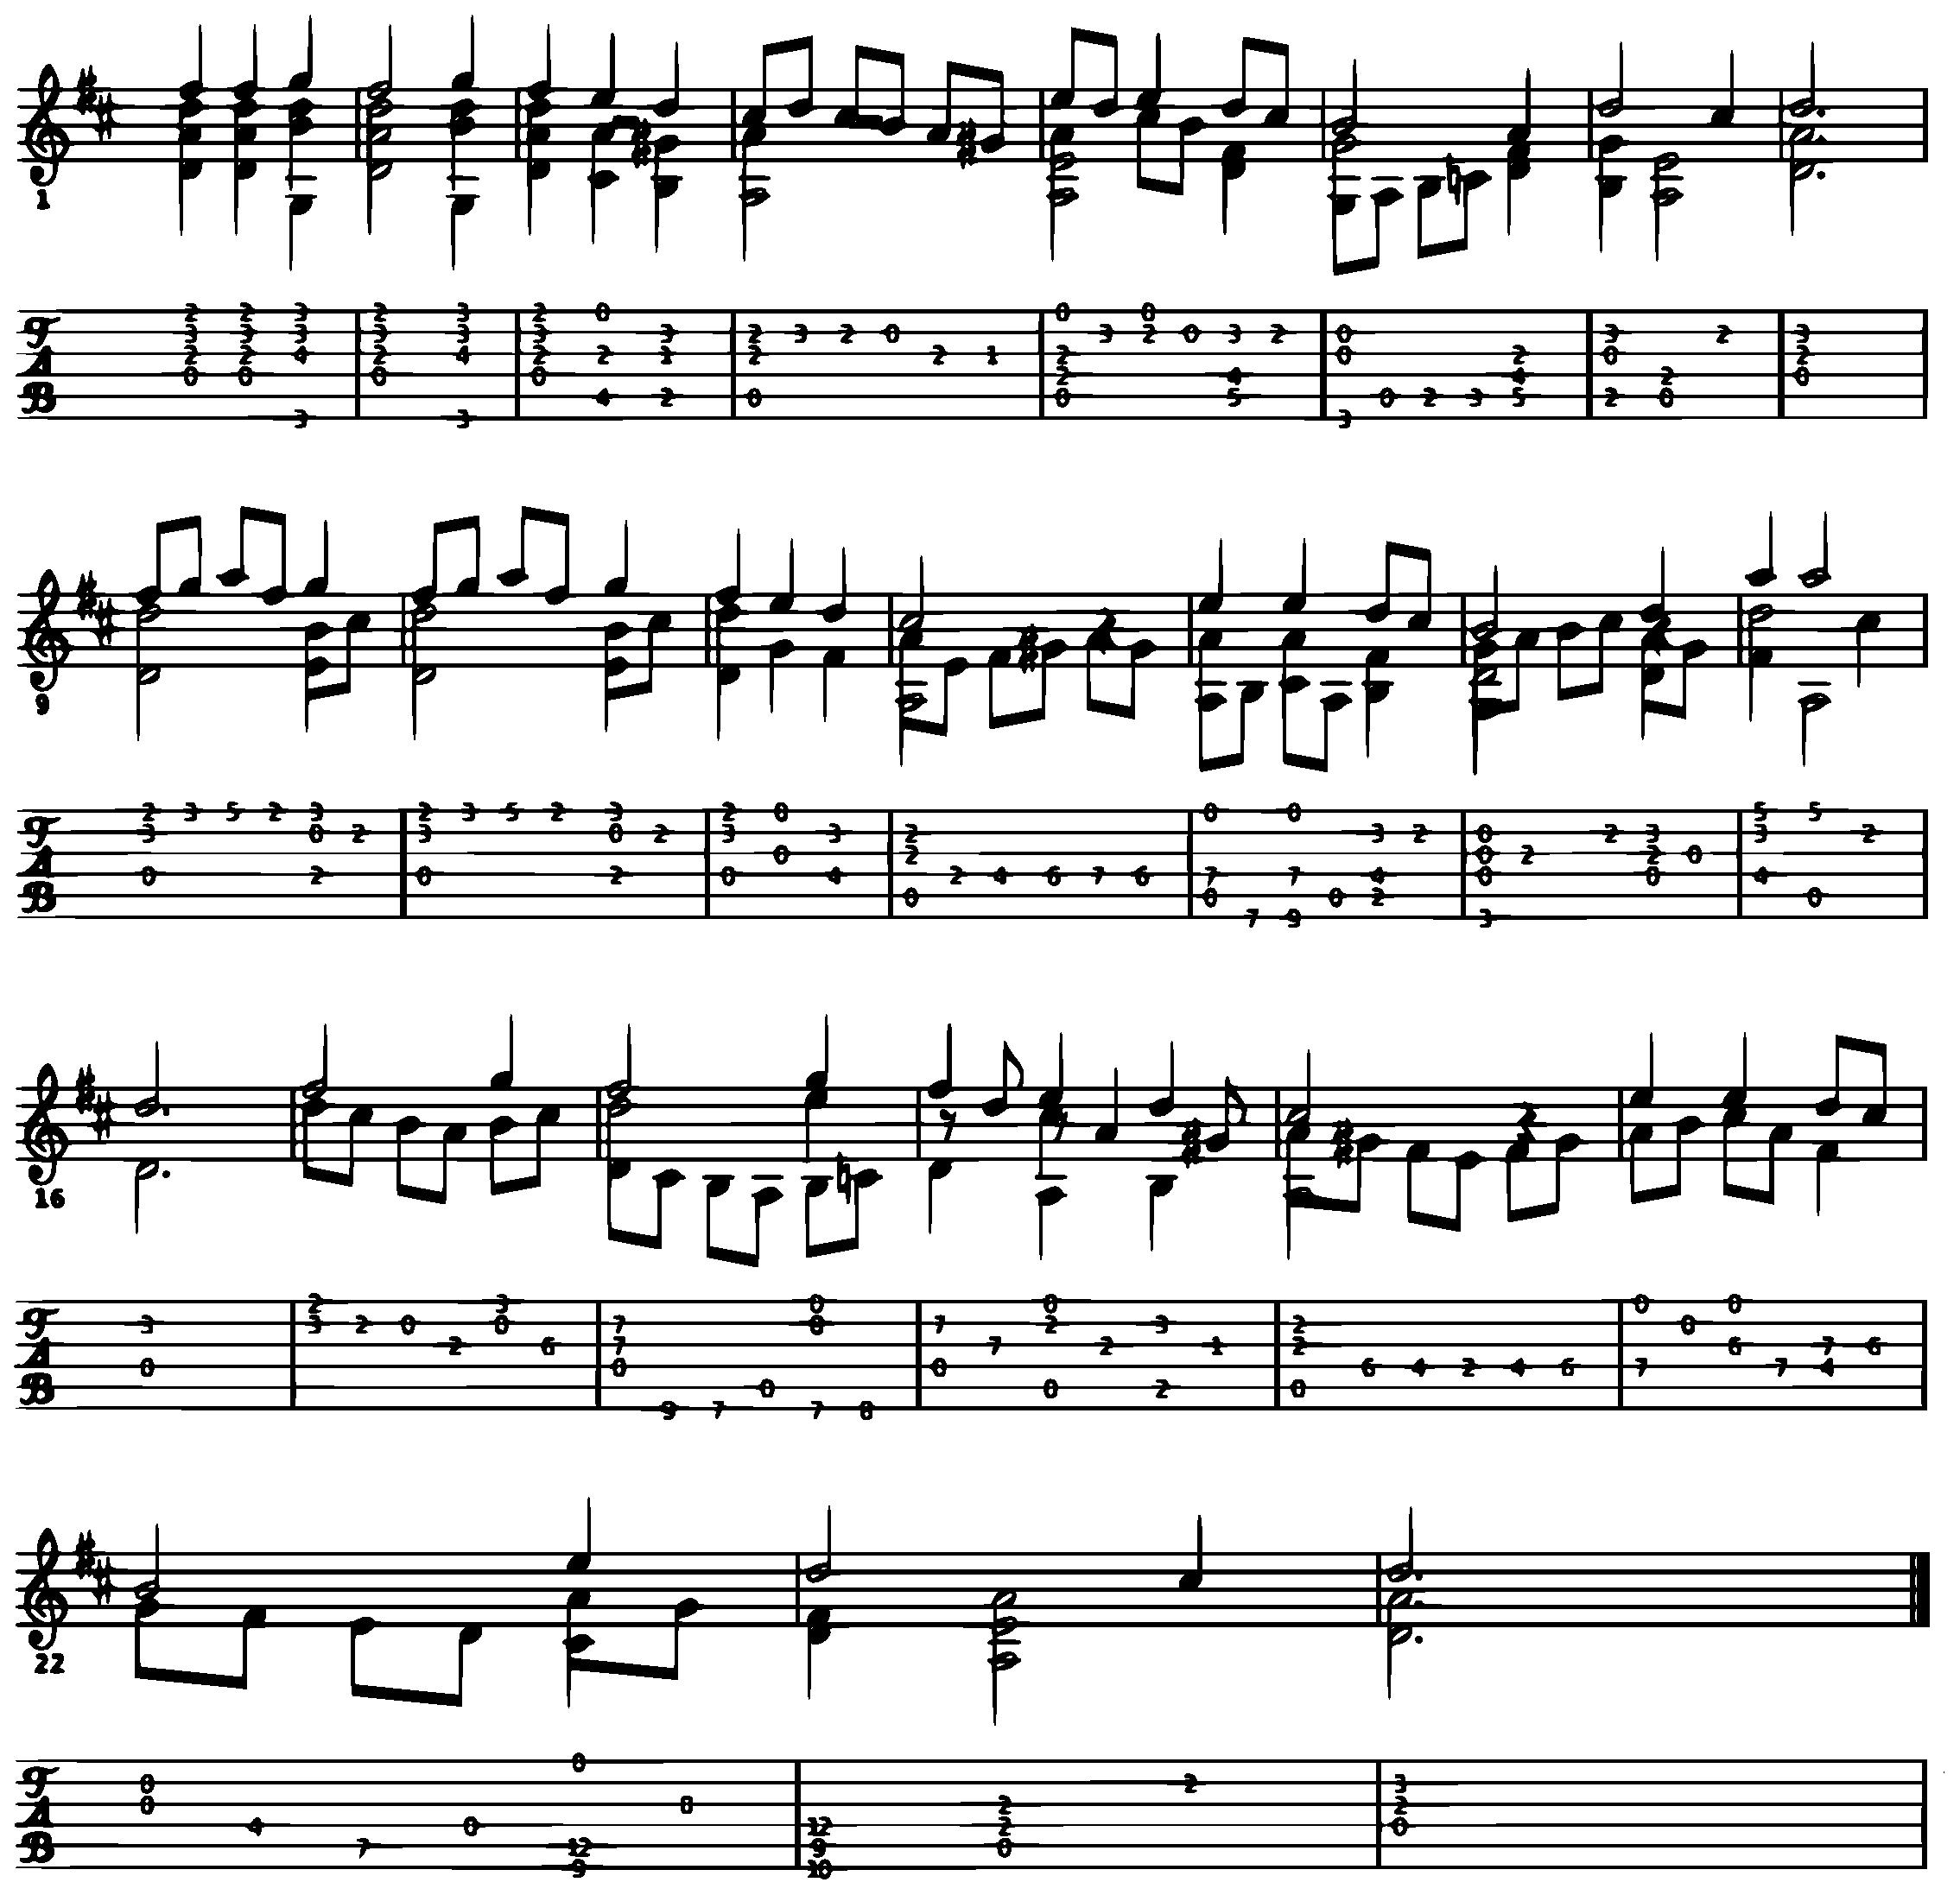
\includegraphics[width=1.0\textwidth]{Figures/Pav.eps}
    \caption{Pavane No.6 for Guitar by Luis Milan}
    \label{fig:result-pav}
\end{figure}
